O dispositivo escolhido para a implementa��o do algoritmo Radix-2 � o  \textit{ZynqBerry - TE0726} da fabricante \textit{Trenz Eletronic$^\circledR$}, apresentado na figura (\ref{fig:ZynqBerry-TE0726}). Este dispositivo � baseado no SoC (\textit{System On Chip}) Raspberry Pi modelo 2, e vem equipado com uma FPGA SoM (\textit{System on Module}) XC7Z010-1CLG225C-REV3, da fam�lia Zynq-700 fabricada pela \textit{Xilinx$^\circledR$} \cite{trenz}. 

\vspace{6mm}
\begin{figure}[H]
	\centering
	\captionsetup{width=0.6\textwidth, font=footnotesize, textfont=bf}	
	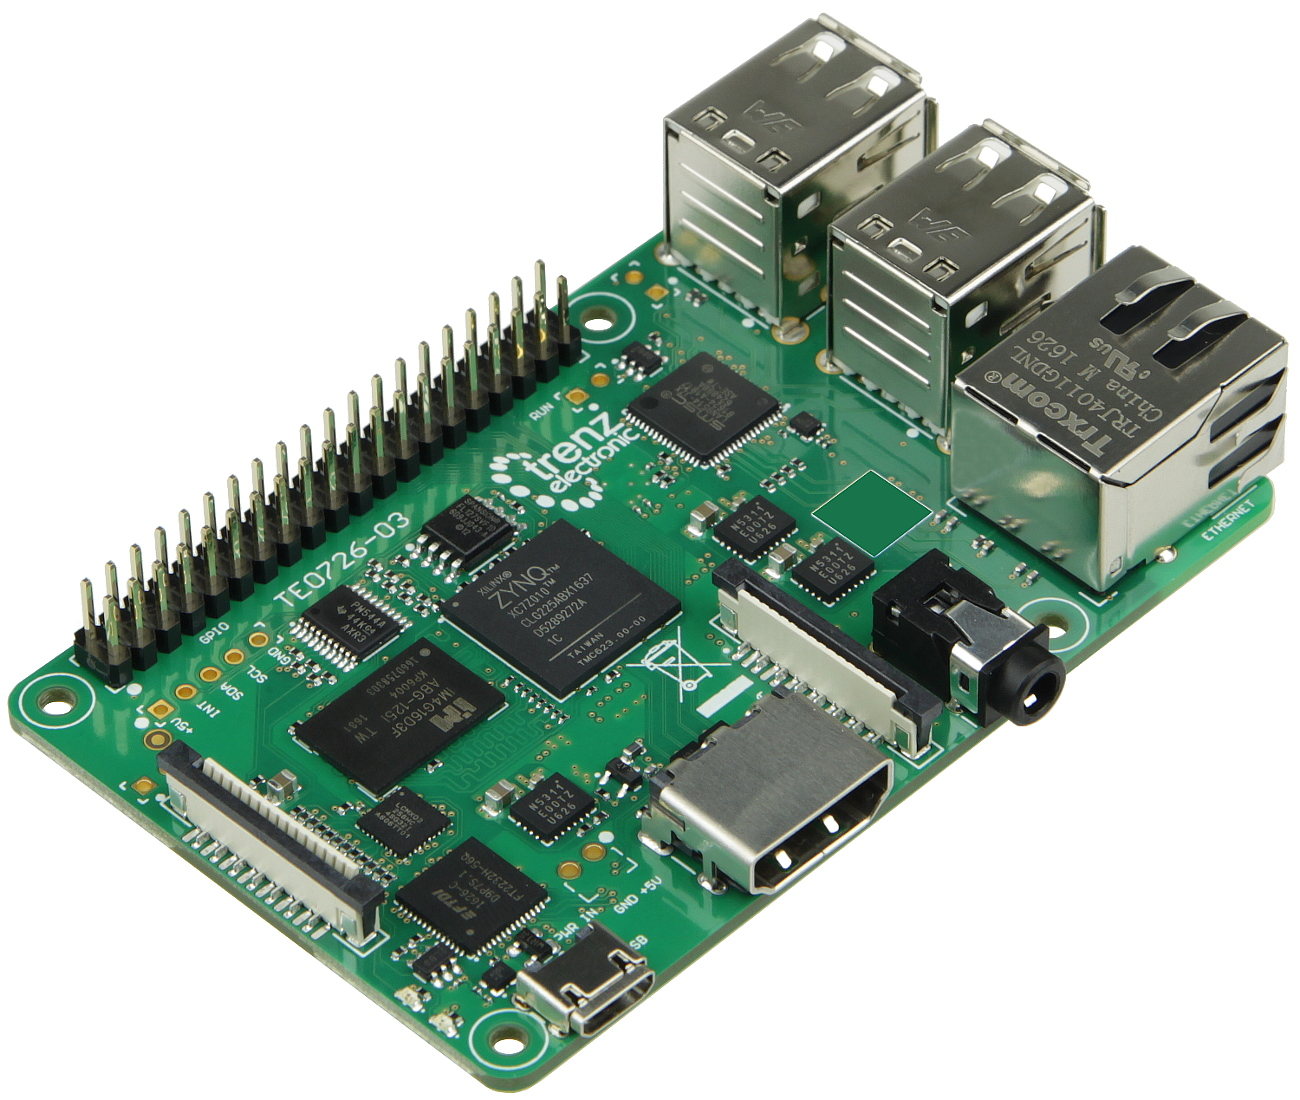
\includegraphics[width=0.6\linewidth]{Images/MateriaisMetodos/TE0726-03M_0.jpg}
	\caption{SoC ZynqBery - TE0726}
	\vspace{-3.5mm}
	\caption*{Fonte: \citeonline{trenz}}
	\label{fig:ZynqBerry-TE0726}
\end{figure}
\vspace{6mm}


A FPGA XC7Z010-1CLG225C tem a mesma arquitetura dos modelos da fam�lia Artix-7, tamb�m da Xilinx, e cont�m recursos como: 28.000 c�lulas l�gicas, 17.600 LUTs, 2.1 Mb de mem�ria RAM divididos em blocos de 26Kb e um total de 36.200 \textit{flip-flops}. Cada CLB, nesta FPGA, para implementar diferentes opera��es l�gicas, utiliza 16 \textit{flip-flops}, 2 somadores de 4 \textit{bits} cascate�veis e ainda 8 LUTs. Sendo poss�vel configurar a memoria RAM das LUTs para 64x1 ou 32x2 bits, ou ainda como um  \textit{shift register (SRL)}. Al�m disso, esta FPGA possuir 80 blocos DSP, cada um equipado com um multiplicador simples de 18x25, e um somador/acumulador de 48 bits \cite{zynq-7000}. Todas estes recursos fazem do XC7Z010 um \textit{hardware} competente para as mais diversas aplica��es de processamento de sinais, como o calculo da FFT.

O processador utilizado no ZynqBerry TE0726-03M � um dual-core ARM Cortex-A9 de 866MHz, que proporciona um desempenho significativo em Sistemas Operacionais \sigla[Sistema Operacional]{S.O.},  como o sistemas baseados em kernel Linux, que podem incluem interface gr�fica sofistica. Cada n�cleo deste processador conta ainda uma unidade NEON\texttrademark  Media Processing Engine (MPE), para alto desempenho em codifica��o e decodifica��o de �udio e v�deo, e uma unidade de ponto flutuante para incremento da precis�o em opera��es matem�ticas \cite{zynq-7000}.  Aliando a versatilidade da XC7Z010 e o poder de processamento do ARM Cortex-A9, � poss�vel construir um sistema que execute uma vers�o do S.O. Linux, tirando proveito de toda a funcionalidade de tal sistema operacional pode prover, e que ainda disponha de um \textit{hardware} acelerador personalizado para aplica��es espec�ficas, trabalhando com paralelismo em alta frequ�ncia. Provendo assim uma solu��o engenhosa de alto desempenho para processamento de sinais.

Para a implementa��o das FFTs realizadas neste trabalho, utilizando o XC7Z010-1CLG225C, foi necess�rio realizar a programa��o l�gica da FPGA (PL), implementando os circuitos l�gicos da arquitetura, e ainda programar o Sistema de Processamento (PS), com as rotinas de envio e recebimento de dados Via UART. O processo de programa��o de ambas partes PL e PS, podem ser vistas no Anexo (\ref{cap:MapeantoProgZynq})